
% VLDB template version of 2020-08-03 enhances the ACM template, version 1.7.0:
% https://www.acm.org/publications/proceedings-template
% The ACM Latex guide provides further information about the ACM template

\documentclass[sigconf, nonacm]{acmart}
\usepackage{graphicx} % Required for inserting images
\usepackage{amsmath}
\usepackage[margin=1cm]{geometry}

%% The following content must be adapted for the final version
% paper-specific
\newcommand\vldbdoi{XX.XX/XXX.XX}
\newcommand\vldbpages{XXX-XXX}
% issue-specific
\newcommand\vldbvolume{14}
\newcommand\vldbissue{1}
\newcommand\vldbyear{2020}
% should be fine as it is
\newcommand\vldbauthors{\authors}
\newcommand\vldbtitle{\shorttitle} 
% leave empty if no availability url should be set
\newcommand\vldbavailabilityurl{URL_TO_YOUR_ARTIFACTS}
% whether page numbers should be shown or not, use 'plain' for review versions, 'empty' for camera ready
\newcommand\vldbpagestyle{plain} 

\begin{document}
% \title{A Relational Model of Data for Large Shared Data Banks}
\title{CogSci 131: Back Propagation}
% \author{Chanwut (Mick) Kittivorawong\\SSID: 3037251249}
% % \date{September 2025}

%%
%% The "author" command and its associated commands are used to define the authors and their affiliations.
\author{Chanwut (Mick) Kittivorawong\\SSID: 3037251249}
% \affiliation{%
%   \institution{Institute for Clarity in Documentation}
%   \streetaddress{P.O. Box 1212}
%   \city{Dublin}
%   \state{Ireland}
%   \postcode{43017-6221}
% }
% \email{trovato@corporation.com}

\maketitle

\section{Neural Network Diagram}
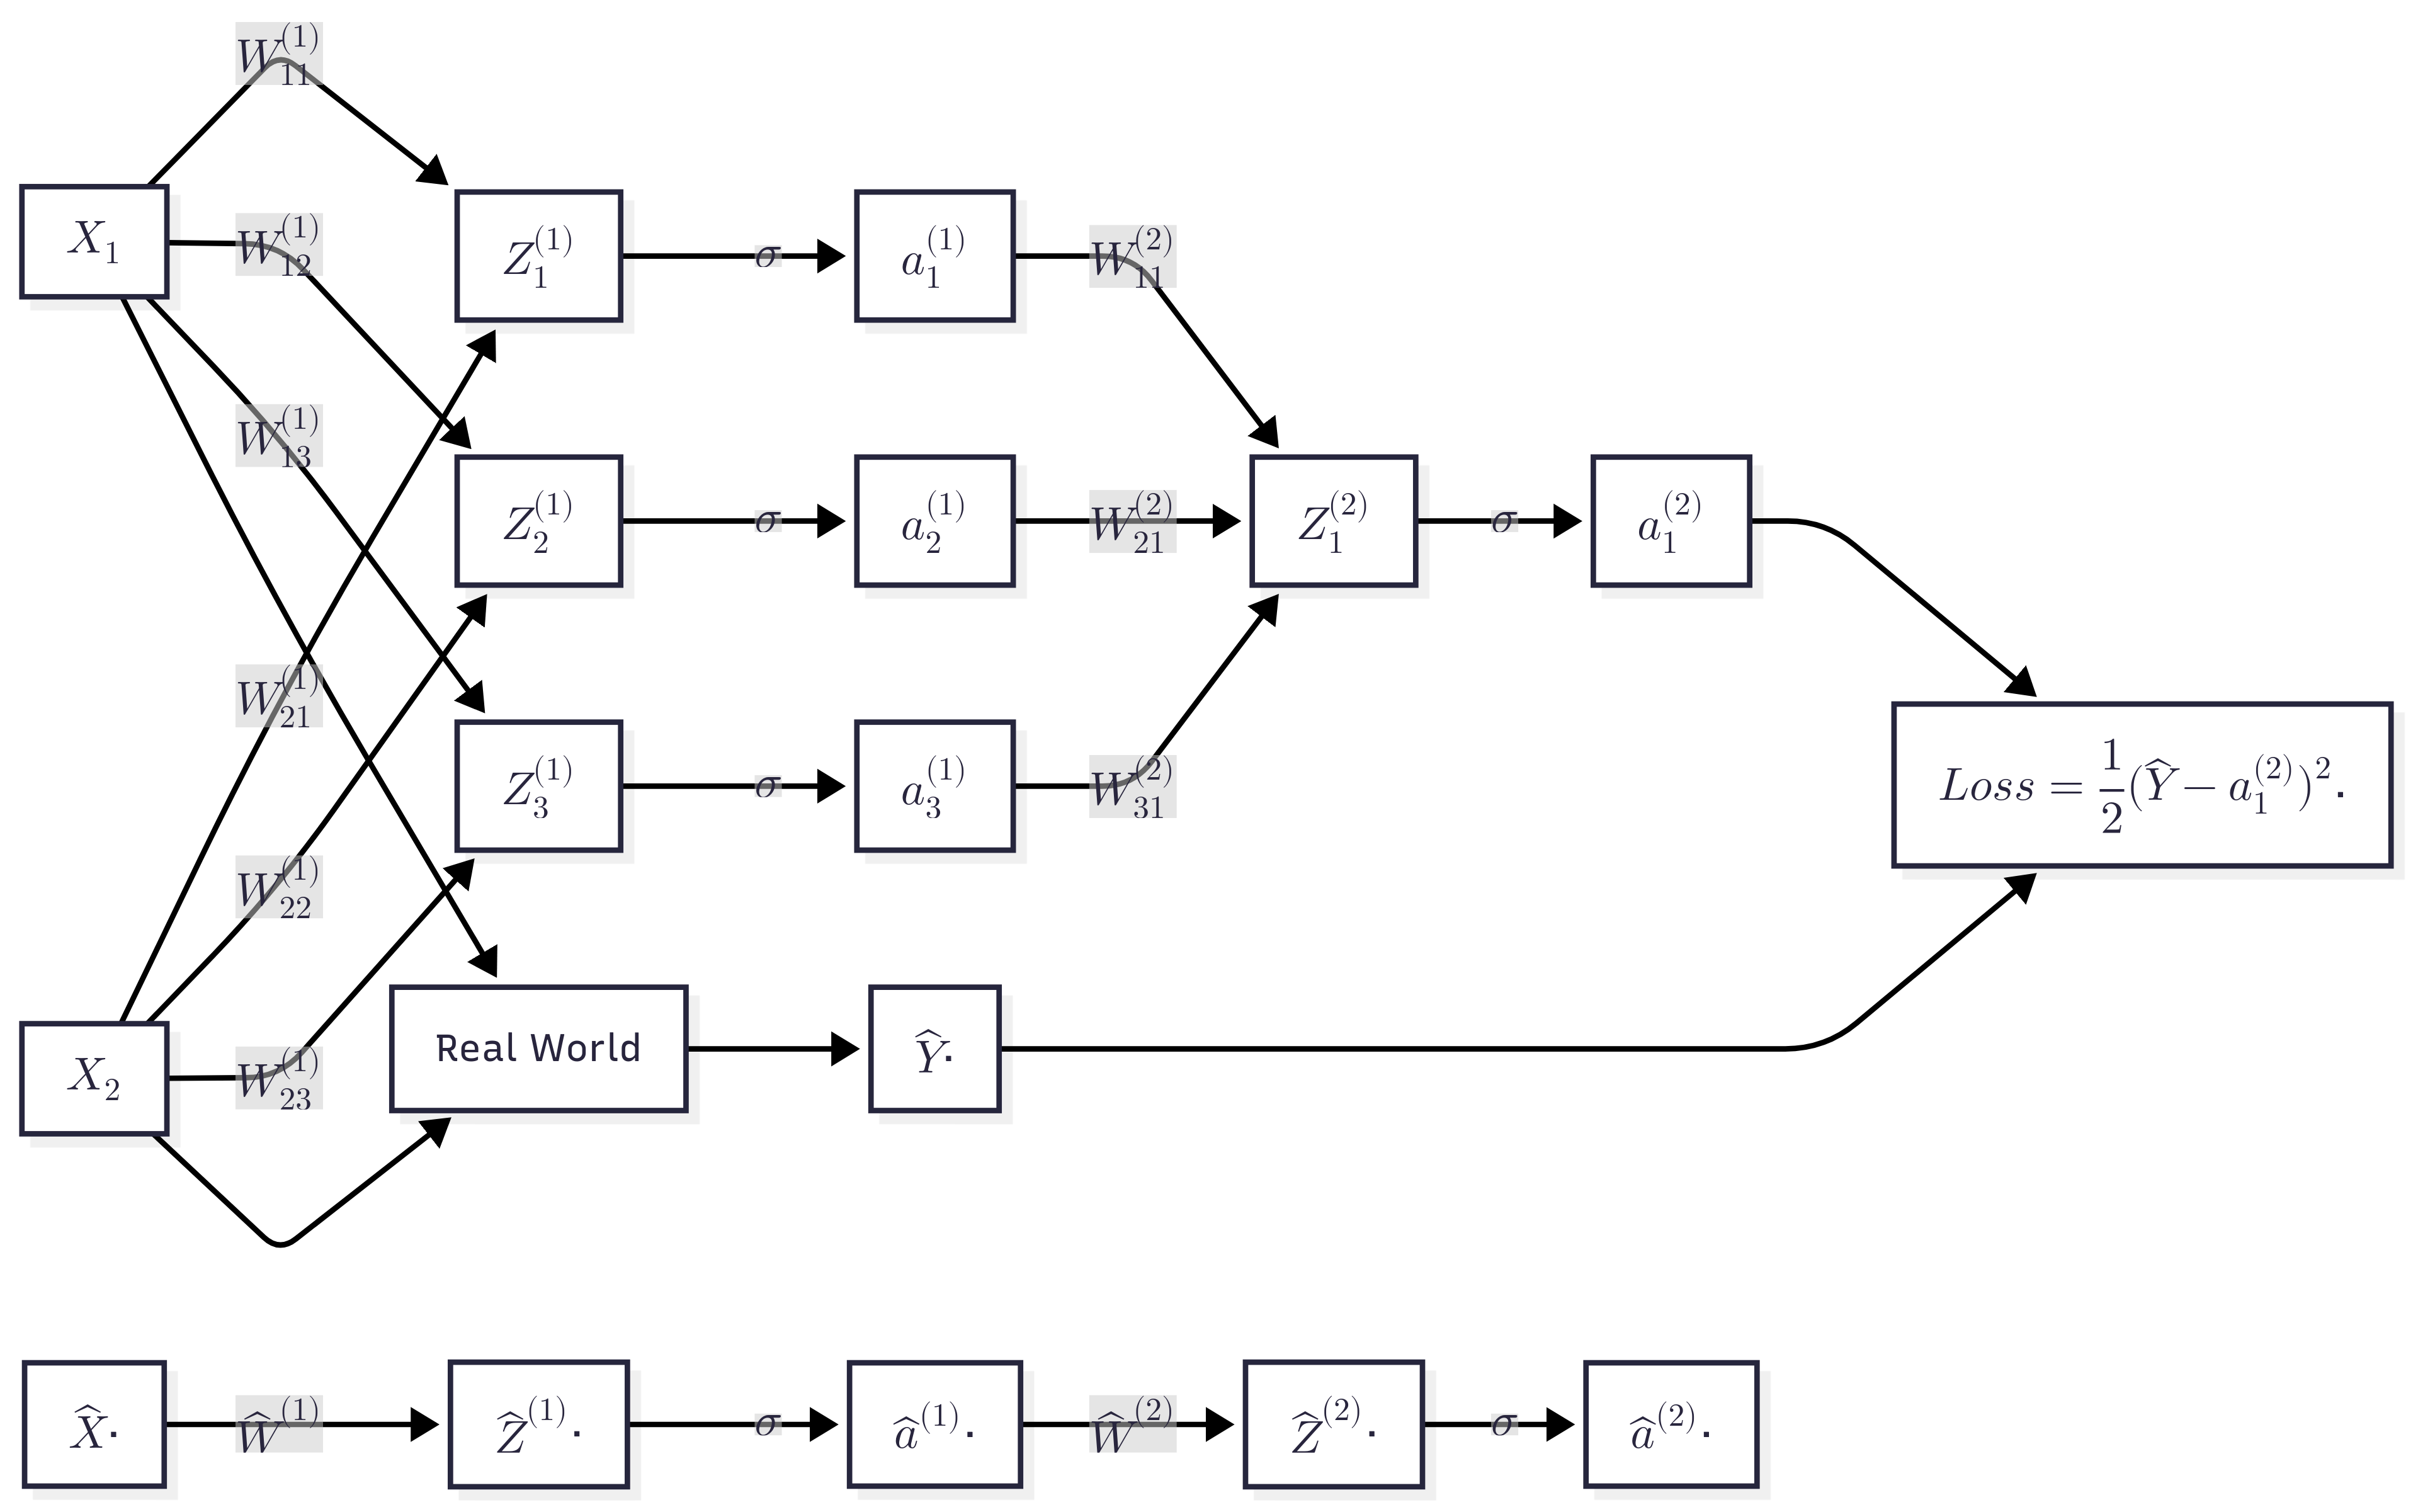
\includegraphics[width=\textwidth]{nn.png}

\section{All variables}
Below are all the variables in the neural networks.\\

\begin{tabular}[h]{l l l l}
{
$\hat{X} = \begin{pmatrix}
X_1 &
X_2
\end{pmatrix}$
} & {
$\hat{W}^{(1)} = \begin{pmatrix}
W^{(1)}_{11} & W^{(1)}_{12} & W^{(1)}_{13}\\
W^{(1)}_{21} & W^{(1)}_{22} & W^{(1)}_{23}
\end{pmatrix}$
} & {
$\hat{Z}^{(1)} = \begin{pmatrix}
Z^{(1)}_1 &
Z^{(1)}_2 &
Z^{(1)}_3
\end{pmatrix}$
} & {
$\hat{a}^{(1)} = \begin{pmatrix}
a^{(1)}_1 &
a^{(1)}_2 &
a^{(1)}_3
\end{pmatrix}$
} \\
{
$\hat{W}^{(1)} = \begin{pmatrix}
W^{(1)}_{11}\\
W^{(1)}_{21}\\
W^{(1)}_{31}
\end{pmatrix}$
} & {
$\hat{Z}^{(2)} = \begin{pmatrix}
Z^{(2)}_1
\end{pmatrix}$
} & {
$\hat{a}^{(2)} = \begin{pmatrix}
a^{(2)}_1
\end{pmatrix}$
} & {
$L = \frac{1}{2} (\hat{Y} - a^{(2)}_1)^2$
}
\end{tabular}

\section{Forward Propagation}
\subsection{Layer 1}

\subsubsection{Calculating $\hat{Z}^{(1)}$}
Given $\hat{Z}^{(1)} = \hat{X} \times \hat{W}^{(1)}$\\
Then, $\begin{pmatrix}
Z^{(1)}_1 &
Z^{(1)}_2 &
Z^{(1)}_3
\end{pmatrix} = \begin{pmatrix}
X_1 &
X_2
\end{pmatrix} \times \begin{pmatrix}
W^{(1)}_{11} & W^{(1)}_{12} & W^{(1)}_{13}\\
W^{(1)}_{21} & W^{(1)}_{22} & W^{(1)}_{23}
\end{pmatrix}$\\
Thus,
$Z^{(1)}_{i} = \sum_{j=1}^{j \le 2} X_j W^{(1)}_{ji}$

\subsubsection{Calculating $\hat{a}^{(1)}$}
Given $\hat{a}^{(1)} = \sigma(\hat{Z}^{(1)})$\\
Then,
$a^{(1)}_{i} = \sigma(\sum_{j=1}^{j \le 2} X_j W^{(1)}_{ji})$

\subsection{Layer 2}
\subsubsection{Calculating $\hat{Z}^{(2)}$}
Given $\hat{Z}^{(2)} = \hat{a}^{(1)} \times \hat{W}^{(2)}$\\
Then, $\begin{pmatrix}
Z^{(2)}_1
\end{pmatrix} = \begin{pmatrix}
a^{(1)}_1 &
a^{(1)}_2 &
a^{(1)}_3
\end{pmatrix} \times \begin{pmatrix}
W^{(2)}_{11}\\
W^{(2)}_{21}\\
W^{(2)}_{31}
\end{pmatrix}$\\
Thus,
$Z^{(2)}_{1} = \sum_{i=1}^{i \le 3} a^{(1)}_i W^{(2)}_{i1}$

\subsubsection{Calculating $\hat{a}^{(2)}$}
Given $\hat{a}^{(2)} = \sigma(\hat{Z}^{(2)})$\\
Then,
$a^{(2)}_1 = \sigma(\sum_{i=1}^{i \le 3} a^{(1)}_i W^{(2)}_{i1})$

\subsection{Loss}
\begin{align*}
L &= \frac{1}{2}(\hat{Y} - \sigma(\sum_{i=1}^{i \le 3} a^{(1)}_i W^{(2)}_{i1}))^2\\
 &= \frac{1}{2}(\hat{Y} - \sigma(\sum_{i=1}^{i \le 3} \sigma(\sum_{j=1}^{j \le 2} X_j W^{(1)}_{ji}) W^{(2)}_{i1}))^2
\end{align*}


\section{Backward Propagation}
\subsection{Layer 2}

%\clearpage

% \bibliographystyle{ACM-Reference-Format}
% \bibliography{sample}

\end{document}
\endinput

% \documentclass[sigconf]{acmart}
% %% \BibTeX command to typeset BibTeX logo in the docs
% \AtBeginDocument{%
%   \providecommand\BibTeX{{%
%     Bib\TeX}}}
% % TODO: use acmart
% \usepackage{graphicx} % Required for inserting images
% \usepackage{amsmath}
% \usepackage[margin=1cm]{geometry}

% \begin{document}

% \title{CogSci 131: Back Propagation}
% \author{Chanwut (Mick) Kittivorawong\\SSID: 3037251249}
% % \date{September 2025}

% \maketitle



% \end{document}